\section{Accessibilità}

\paragraph{Linee guida}

I testi alternativi alle immagini sono stati impostati secondo le seguenti regole:
\begin{itemize}

\item Il testo deve presentare il contenuto e la funzione dell'immagine;
\item Il testo deve essere breve, non più di due sentenze;
\item Evitare di ripetere quanto già riportato nel testo vicino l'immagine;
\item Non iniziare con "immagine di.." o "fotografia di..".
\end{itemize}

\subsection{Accessibilità sezione pubblica}

\paragraph{Cecità ai colori}
Per testare che il sito sia accessibile alle persone daltoniche, tetracromiche o con altri problemi riguardanti i colori si è utilizzato l'estensione Vischeck, scaricabile dal sito Vischeck.com. Tale estensione, eseguibile con ImageJ, data un'immagine o una pagina web, mostra come viene percepita da chi soffre di cecità ai colori. È bastato verificare un paio di pagine, in quanto i colori e le immagini di background utilizzate sono le medesime in tutte le pagine.

\begin{figure}[H]
		\centering 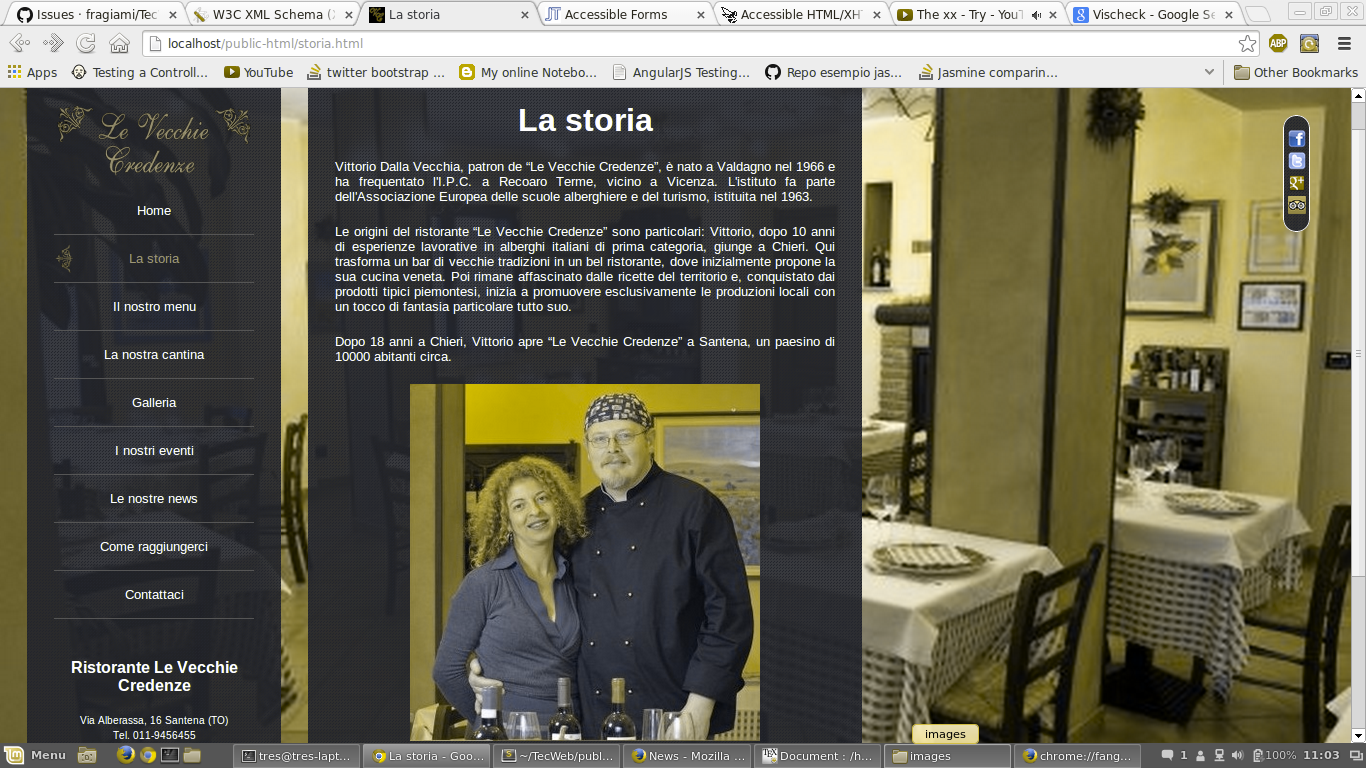
\includegraphics[width=0.8\textwidth]{images/color1.png}
		\caption{Esempio di pagina vista da chi soffre di deuteranopia}
\end{figure}
	
\begin{figure}[H]
		\centering 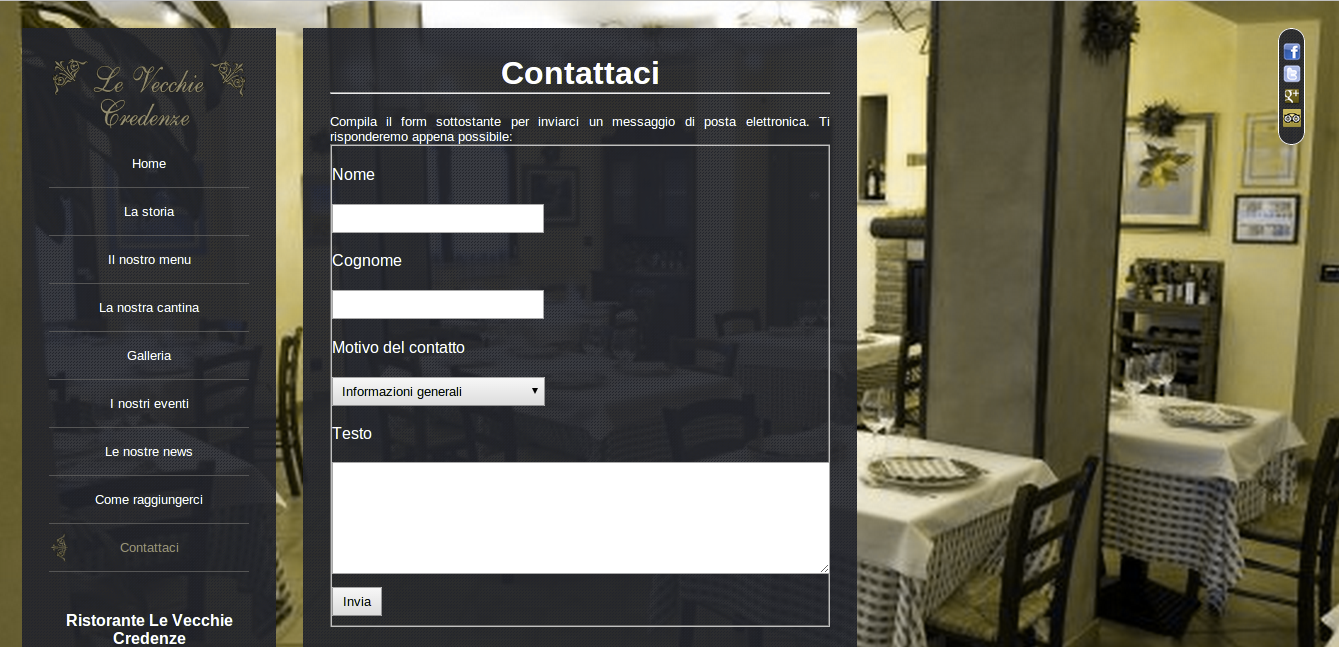
\includegraphics[width=0.8\textwidth]{images/color2.png}
		\caption{Esempio di pagina vista da chi soffre di protanopia}
\end{figure}
	
\begin{figure}[H]
		\centering 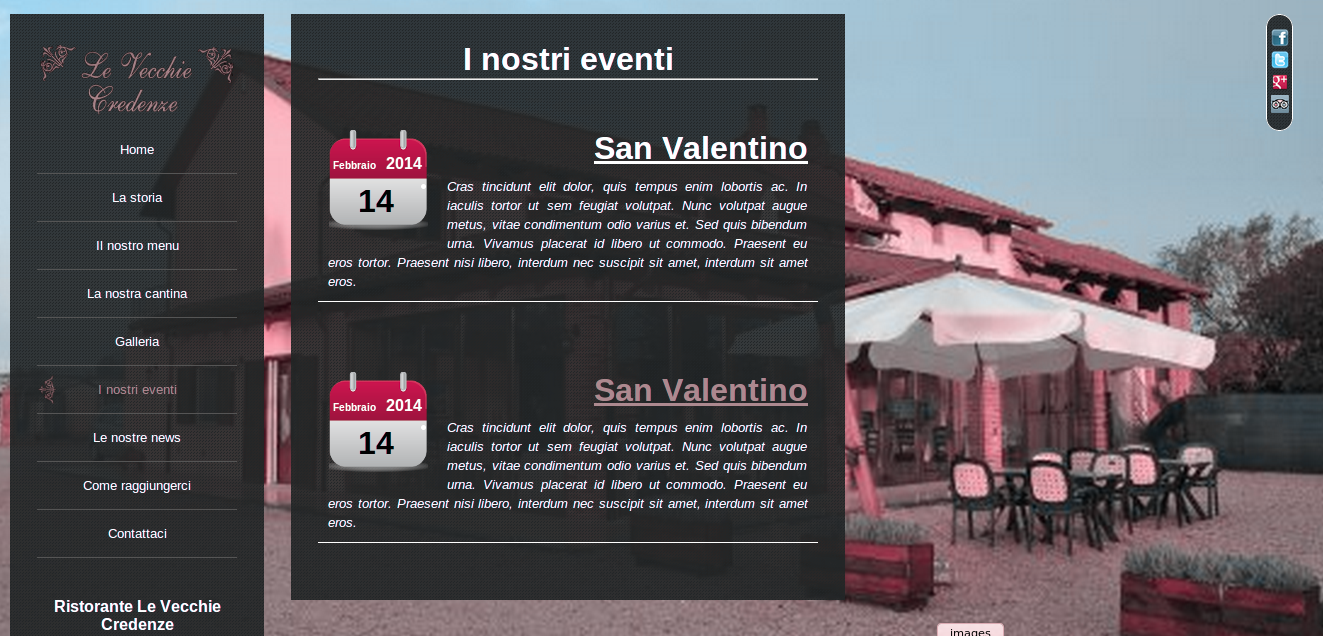
\includegraphics[width=0.8\textwidth]{images/color3.png}
		\caption{Esempio di pagina vista da chi soffre di tritanopia}
\end{figure}


\paragraph{Utilizzo della sola tastiera}
Per essere accessibile un sito deve poter essere navigabile utilizzando solamente la tastiera. 
Ogni pagina è stata testata ed il risultato è che l'intero sito è navigabile utilizzando \emph{Tab} ed \emph{Enter}.
Non sono stati utilizzati gli attributi \emph{tabindex} per i link in quanto il flusso logico del sito è semplice e lineare.

\paragraph{Cecità}
Per testare il sito rispetto agli \emph{screen reader} è stata utilizzata l'estensione \emph{Fangs} del browser Firefox.
Tale estensione simula come un generico screen reader interpreta le varie pagine. 
Un problema che è sorto è stata la mancanza dell'italiano tra le lingue supportate da Fangs. Nonostante ogni pagina indichi l'italiano come lingua di default, tramite l'attributo \emph{lang}, Fangs imposta l'inglese come lingua di default, e ad esempio legge i numeri decimali come centinaio (Ecco nella pagina cantina 2,00 diventa two hundred).

Nonostante ciò Fangs ha permesso di verificare che:
\begin{itemize}
\item tutti i link vengano catturati, e che ogni link abbia un significato chiaro;
\item cambi lingua, le abbreviazioni e le tabelle fossero gestiti correttamente;
\item visualizzare gli headers della pagina, funzionalità offerta da alcuni scree reader e utile per capire a grandi linee il contenuto della pagina e la sua struttura. Un esempio dell'utilità di tale funzionalità è data dalla pagina news, in cui grazie agli header è possibile accedere immediatamente ai titoli di tutte le news presenti, per poi selezionare quella di proprio interesse.s
\item Ogni immagine abbia il rispettivo testo alternativo.
\end{itemize} 

\begin{figure}[H]
		\centering 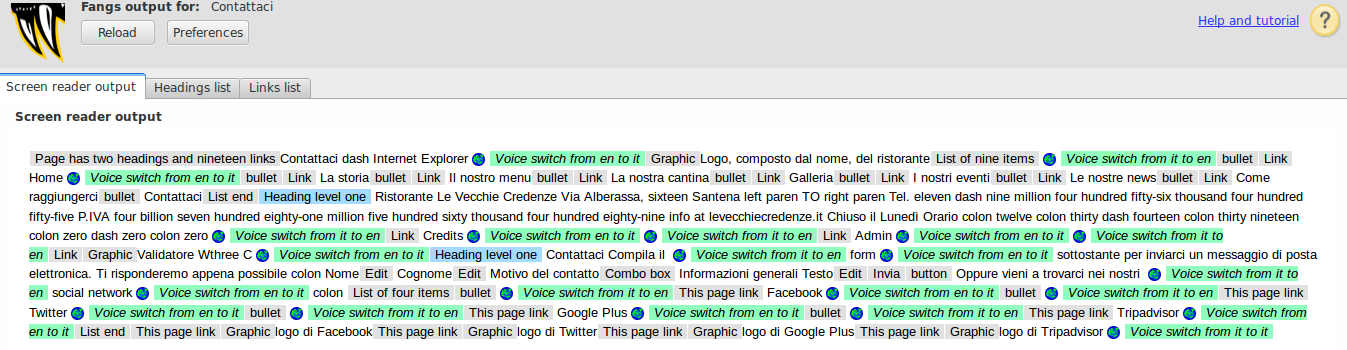
\includegraphics[width=0.8\textwidth]{images/fangs.png}
		\caption{Output di Fangs}
	\end{figure}
	
	\begin{figure}[H]
		\centering 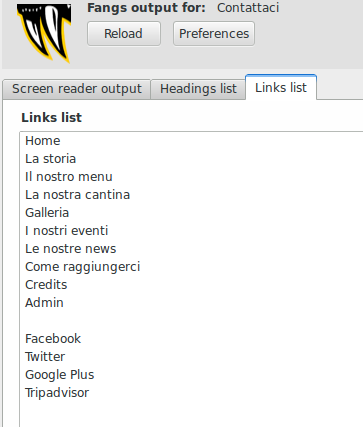
\includegraphics[width=0.8\textwidth]{images/fangsLink.png}
		\caption{Elenco di link della pagina, come visualizzati da Fangs}
	\end{figure}

\paragraph{Accessibilità dei form}

Possiamo vedere un esempio di accessibilità dei form nella pagina contatti.html.

Per chi utilizza uno screen reader, nel compilare un form è fondamentale sapere come compilare gli input. Per questo motivo ad ogni \emph{input type text} è associata una label con attributo for, il cui valore è l'id dell'input a cui fa riferimento. Con questa tecnica lo screen reader sa certamente collegare nel modo corretto un'input alla sua label.
Tale tecnica è stata utilizzata anche per i \emph{select menus}

Per ogni bottone è stato utilizzato il tipo submit in quanto button necessita che javascript sia bilitato per funzionare, inoltre in ogni bottone è stato valorizzato l'attributo value, in modo che lo screen reader dia un significato esplicito all'azione del bottone.

\paragraph{Total Validato}
Total validator è uno strumento, che tramite un'apposita estensione di Firefox permette di verificare l'accessibilità di una pagina web secondo alcuni parametri.
Le impostazioni di total validator scelte sono le più stringenti, richiedendo un'accessibilità aderente allo standard WCAG 2.0 AAA.
Di seguito sono riportati alcuni errori segnalati da total validator, ma non corretti per i motivi riportati.\\ \\
\textbf{Pagina} storia.html \\
\textbf{Riga: Errore} 63: The 'alt' attribute is for short descriptions. Use 'longdesc' for long ones. \\ \\
Non è stato utilizzato longdesc per due motivi:
\begin{itemize}
\item Non è supportato da tutti gli screen reader;
\item Il valore di tale attrivuto solitamente è un link ad un'altra pagina, anche esterna al sito che contiene la descrizione dell'immagine, e non un testo descrittivo.
\end{itemize}

\subsection{Accessibilità sezione amministrazione}
A differenza della parte pubblica del sito per poter usufruire della parte privata è necessario aver abilitato Javascript sul browser, le ragioni di tale scelta si possono identificare nel fatto che a seguito dell' analisi dell' utenza effettuata si è ritenuto che l' amministratore non disattivi mai javascript. Nonostante sia un progetto didattico è stato dimostrato che il gruppo sa gestire il caso in cui l' utente disattivi javascript nella parte pubblica.
\paragraph{Accessibilità dei form}
Per quanto riguarda l' accessibilità dei vari form, si è deciso di adottare questi accorgimenti:
\begin{itemize}
 \item in ogni label di ogni input text obbligatoria sarà presente il carattere *, il quale viene letto dagli screen reader che notificano all' utente che il campo è un campo obbligatorio come si può notare dall' immagine "screen reader required input";
 \item nel caso in cui si cerchi di inserire un carattere diverso da un numero o da delete all' interno dei campi che richiedono un numero, verrà impedito e l' utente verrà avvisato che si possono inserire solo numeri;
 \item se l' amministratore cercherà di inviare un form, nel quale non si siano riempiti campi obbligatori, l' azione verrà bloccata, evidenziando ogni input text non riempita correttamente con un' aura rossa intorno ad essa rendendo evidenti i campi vuoti. L' aura è volutamente molto larga in quanto dopo aver testato con vischeck si è ritenuta efficace questa ampiezza, inoltre il colore è accessibile in presenta di cecità ai colori. Quando si andrà a inserire un valore valido in uno di questi campi evidenziati si andrà a rimuovere l' aura dall' input text.
 \item per gli utilizzatori di screen reader, la compilazione necessita di label con un campo for adeguato per sapere come compilare una input text, e ciò è stato implementato in tutti i form della parte privata, anche in quelle sezioni dove i campi verranno aggiunti dinamicamente con l' uso di Jquery si è prestata attenzione a creare id adeguati e diversi per ogni campo e assegnarlo in modo corretto alla rispettiva label;
\end{itemize}
\begin{figure}[H]
		\centering 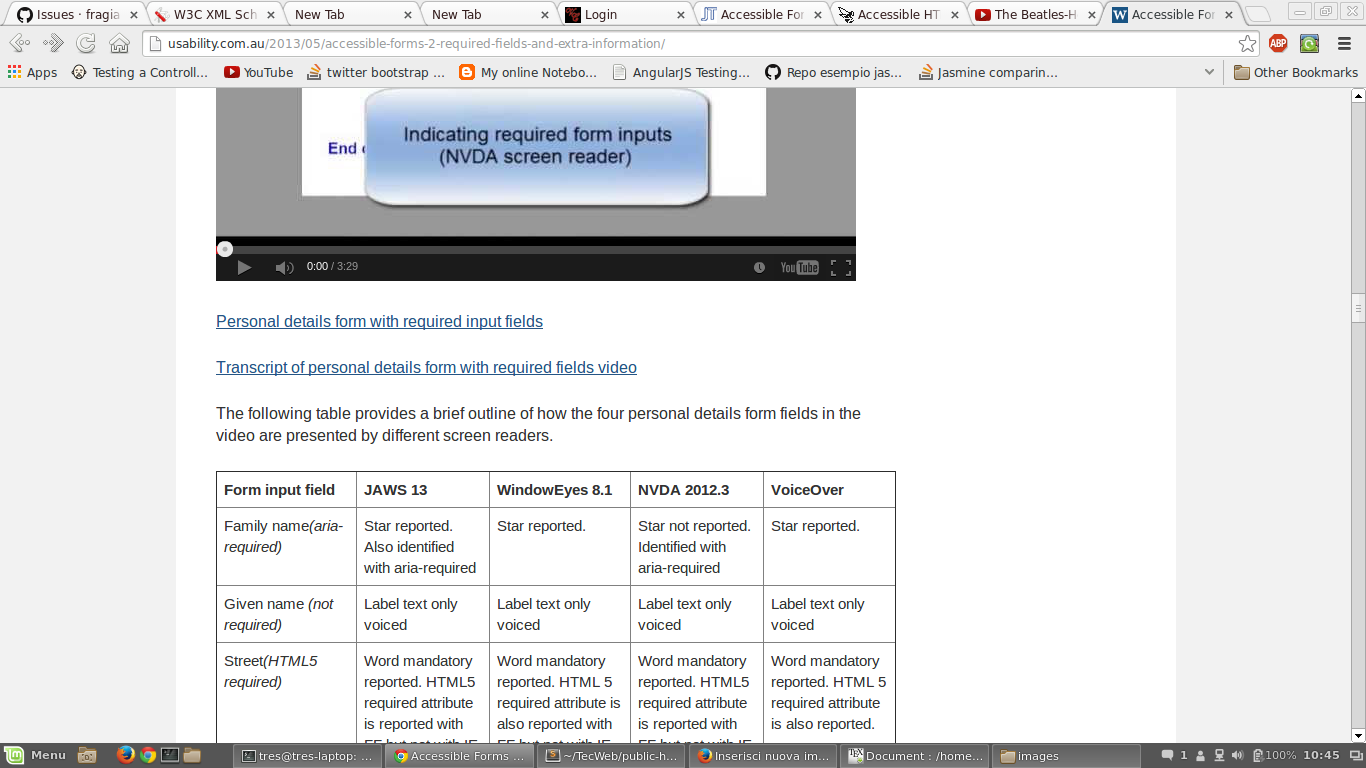
\includegraphics[width=0.8\textwidth]{images/required.png}
		\caption{"screen reader required input" reazioni degli screeen reader a *}
	\end{figure}
	\begin{figure}[H]
		\centering 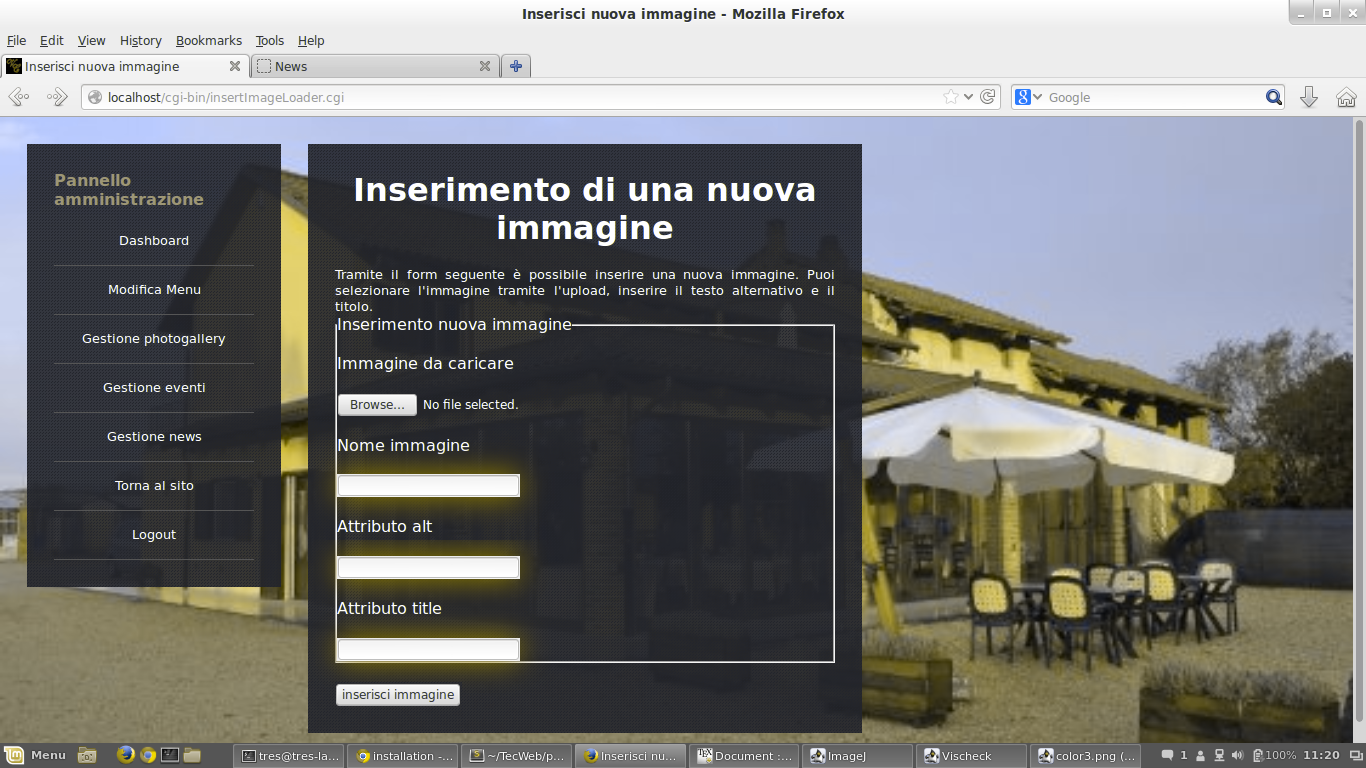
\includegraphics[width=0.8\textwidth]{images/color4.png}
		\caption{aura intorno ai campi lasciati vuoti vista in presenza di cecità ai colori}
	\end{figure}
\paragraph{Accessibilità da tastiera}
L' intera parte privata è stata sviluppata in modo da poter essere interamente navigabile solamente con l' uso della tastiera, muovendosi con tab e selezionando gli elementi con invio.
